
\documentclass[]{article}

\usepackage[margin=1in]{geometry}

\usepackage[]{amsthm}
\usepackage[parfill]{parskip}
\usepackage[]{graphicx}
\graphicspath{{../img/}}

\newtheorem{theorem}{Theorem}
\newtheorem{lemma}{Lemma}
\newtheorem{corollary}[]{Corollary}

\title{CMSC 510: BFS \& DFS --- Runtime and Correctness}
\author{Acacia Ackles}

\begin{document}

\maketitle

\section*{Introduction}

We've looked at the pseudocode for our two search algorithms and written them up ourselves. We also tried a few examples on these algorithms, so it feels like they \textit{should} work. But we should prove that first. 

We also might want to know how efficient these algorithms are; after all, there's many ways to search a graph, so how do we know that this is a good way to do so? 

\section*{Analysis of Runtime}

\subsection*{Breadth-First Search}

Let's return to the pseudocode for BFS.

\begin{figure}[h]
    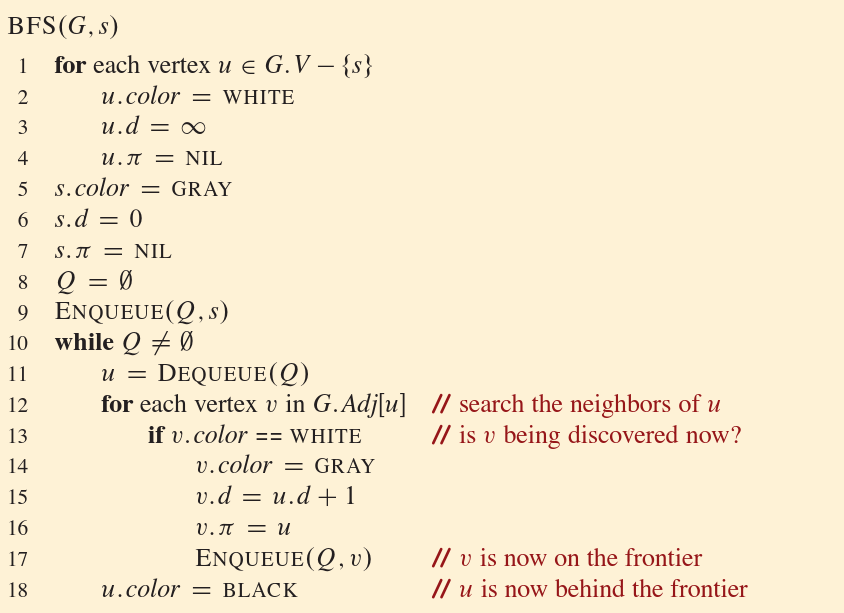
\includegraphics[width=\textwidth]{bfs-pseudocode.png}
\end{figure}

Remember that lines 1 - 8 are effectively initialization steps to set up the grpah, so we'll start in the meat of the algorithm, inside the while loop that begins at line 10. 

How many times will the dequeue operation execute? Perhaps an easier question: how many times will the enqueue operation execute?

Since the algorithm never turns vertices from black back to white, we know that enqueue will happen once for every vertex in the graph. Queueing and dequeueing is constant-time; therefore, the total time to queue and dequeue is $O(V)$. 

The only other looping procedure is the scan of each adjacency list in line 12. It only does this operation when a vertex is dequeued; therefore, it will scan every adjacency list at most one time. This \textit{at most} is important; sometimes, it will just look at the adjacency list and not scan it. 

Thhis scanning of vertex adjacency lists means every list (so, every edge) will be visited at most twice, and every vertex (so, every entry in the list) will be looked at at most once. So the runtime is $O(V+E)$. Be carefuly not to confuse this with the space complexity, which is $V \times E$. 

Nowe we can return to the initialization step to see how long that takes; it basically consists of looking at every vertex to paint it white, and those are constant-time operations. Therefore, it is $O(V)$. 

Our final runtime for the various pieces of this algorithm are then $O(V) + O(V) + O(V+E)$, which simplifies to $O(V+E)$. 

\subsection*{Depth-First Search}

Here is the pseudocode for DFS.

\begin{figure}[h]
    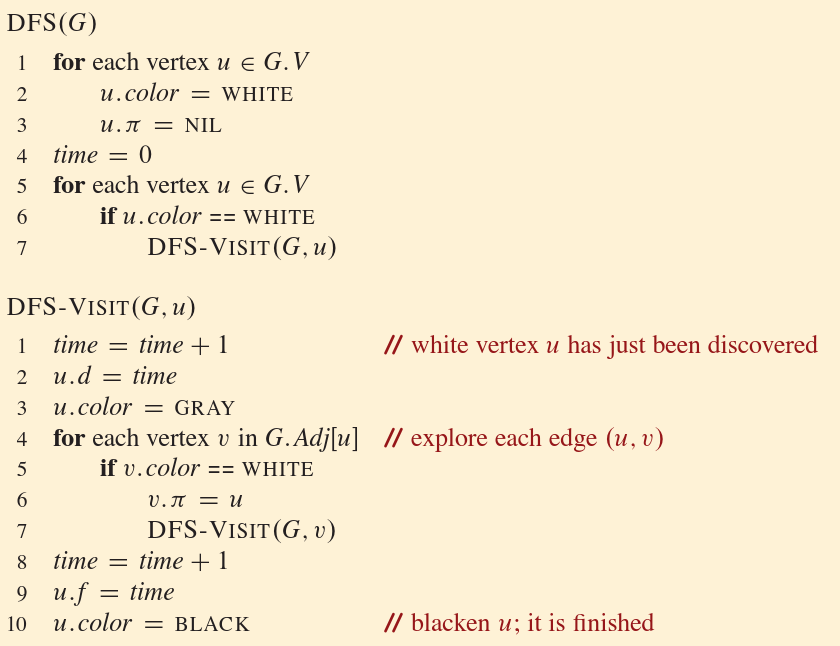
\includegraphics[width=0.75\textwidth]{dfs-pseudocode.png}
\end{figure}

Try to perform a similar runtime analysis on this code. Here are some hints:

\begin{itemize}
    \item Analyze the code irrespective of the recursive call first (i.e. the loops on lines 1-3 and on lines 5-6, ignoring the DFS-VISIT call.)
    \item Before trying to determine the DFS-VISIT runtime, draw a picture of the structure that this code is working through. Use this picture as you are arguing how many times something will be called or executed. 
    \item Next, determine how many times DFS-VISIT will be called during DFS. That is, how many times, at most, will each vertex be visited? 
    \item Finally, determine how many times the loop executes in DFS-VISIT each time it is called. That is, how many times, at most, will each edge be traversed? 
    \item Decide how these last two pieces connect to each other. Just like in BFS, they are not independent! And just like in BFS, do not get space complexity confused with time complexity. A vertex that is done is done; an edge connected to a done vertex can be ignored. 
\end{itemize}

\section*{Proof of Correctness}

\subsection*{Breadth First Search}

The BFS proof of correctness takes on a different style than we have seen before. In this case, we're going to argue through it less like a proof by induction; instead, we we build up some arguments towards the idea that it must visit every vertex by showing that assuming one has been left out would produce a contradiction. 

Here are three Lemmas, the proofs of which are in your book. 


Brief argument for why this is true: The shortest path from $\delta(s,v)$ can't be shorter than the path from $\delta(s,u)$ plus the edge that we know exists from $u$ to $v$. 


From Lemma 3.

Now that we have these lemmas, we can use them to actually build the proof of correctness, which I'll do out in more detail. 

\begin{theorem}
    Let $G = (V,E)$ be a graph. Suppose BFS is run on $G$ from a given source vertex $s$. Then, BFS discovers every vertex reachable from $s$, upon termination $v.d = \delta(s,v)$ for all $v \in V$. Additionally, for any vertex reachable from $s$, one of the shortest paths is a shortest path from $s$ to its predecessor followed by $(v.\pi, v)$
\end{theorem}

Here is the proof. 

Assume for the purposes of contradiction that some vertex receives a $d$ value not equal to its shortest-path distance. 

Is there anything we can say about either $v$ or $\delta(s,v)$? Recall we are trying to prove correctness for an algorithm, so it would be useful to refer to the algorithm to see what we should be doing here. 

We want to see whether $v.d$ accurately contains the shortest possible distance. So what kind of constraint might we be able to put on $v.d$ without proving it directly that helps us towards that goal? 

\begin{lemma}
    Let $G = V(E)$ be a directed or undirected graph, and suppose BFS is run on $G$ from a given source vertes $s \in V$. Then, for each vertex $v \in V$, the value $v.d$ computed by BFS satisfies the following at all times:

    $v.d \geq \delta(s,v)$
\end{lemma}

This seems trivially obvious. The formal proof is by induction.

Lemma 1 tells us that $v.d \geq \delta(s,v)$, so since we have assumed the value is not equal, we know $v.d > \delta(s,v)$. 

We can definitively say that $v \neq s$, because $s.d = 0$ and $\delta(s,s) = 0$, so the inequality would be broken. We also know that $v$ must be reachable from $s$, otherwise its distance would be infinite. Therefore, since it is reachable but isn't $s$, there must be some vertex between $s$ and $v$.

In proofs like this, it's often helpful to be able to show that something is going to break at some point. Here the thing that presumably will break is this shortest path, so we want to say as much as possible about that path. So let's define something that seems possibly trivial. 

\begin{lemma}
    Let $G = V(E)$ be a directed or undirected graph, and let $s \in V$ be an arbitrary vertex. Let $\delta(s, u)$ denote the length of the shortest path from $s$ to $u$. Then, for any edge $(u, v) \in E$,

    $\delta(s,v) \leq \delta(s,u) + 1$
\end{lemma}


Let $u$ be the vertex for which $\delta(s,v) = \delta(s, u) + 1$. 

That's great, but we don't have $\delta(s,v)$ because we assumed we didn't have that to begin with. This is where we make one of those mathematical connections that's difficult to organically explain; it's one of those connections that when you see it you feel really smart.

Let's go back to the beginning of our proof. We chose any vertex $v$ here. Can we make that vertex more specific without losing the core of the proof? 

What we do now is choose the closest $v$ such that the proof is still true. This is fine; there has to be a closest one, and as long as it exists we can use it. We can try playing around with that closest $v$ to see if we can find a contradiction somewhere. 

Since $\delta(s,u) < \delta(s,v)$, and because of how we chose $v$, we have $u.d = \delta(s,u)$. 

Putitng these properties together, we have:

$v.d > \delta(s,v) = \delta(s,u) + 1 = u.d + 1$.

Now, we might feel stuck at this point, but because this is a proof by contradiction, what we're really trying to prove is that that $v.d$ cannot possibly be greater than $u.d + 1$. And keep in mind, If it could be, our code would have to make it that way. 

Here's another leap of logic. What do we ACTUALLY want to show? What we actually want to show is that in our procedure, $u$ would be reached before $v$, and that $v.d$ would be assigned correctly. Both of these cases happen during the dequeuing of $u$ and the enqueuing of $v$. So we want to put as many constraints as we can on this queue. 

\begin{lemma}
    Suppose that during the execution of BFS on $G = (V,E)$, the queue $Q$ contains the vertices $(v_1, v_2, \dots, v_r)$. Then, $v_r.d \leq v_1.d + 1$ and $v_i.d \leq v_{i+1}.d$ for $i \in [1, r-1]$. 
\end{lemma}

Brief argument for why this is true: The proof is induction on the number of queue operations. Induction allows us to see that when we pull something off the front, the thing after it will have the same distance or a distance one greater, keeping the inequality. When we add something to the back, the thing at the front of the queue has just been pulled off, and since the inductive hypothesis has held for all of those elements in the queue, the thing we're adding will have the same distance as the new thing at the front or a distance one greater. 

Anyway, now there's three cases to consider here: $v$ is white, $v$ is grey, or $v$ is black. 

If $v$ is white, then $v.d$ would be set to $u.d + 1$, contradicting the inequality. 

If $v$ is black, then it was already removed from the queue, which means it came before $u$. This is where we have to be careful; it's easy to assume that we already know or proved that it can't, but we have not shown that. The proof to show that is quite involved with inductive properties, so I'm just going to write the theorem for you here and its associated corollary. 

\begin{corollary}
    If $v_i$ is enqueued before $v_j$, then $v_i.d \leq v_j.d$ when $v_j$ is enqueued. 
\end{corollary}

Now we see that if $v$ was enqueued before $u$, then it would have to be the case that $v.d \leq u.d$, contradicting the ineuqality. 

If $v$ is grey, then it was painted grey when some other vertex $w$ was dequeued. Therefore, $v.d = w.d + 1$. However, we know that $w.d \leq u.d$, so $v.d = w.d + 1 \leq u.d + 1$, which again contradicts the inequality. 

All reachable vertices must be discoverable otherwise $v.d > \delta(s.v)$. 

\end{document}